%!TEX root = ../TaxationPlan.tex

We now consider how to implement taxes in a world where the system margin grows over time
according to a deterministic process. In particular, we assume that margin follows

$$M_{t+1} = M_{t} + g M_{t} \left(1 + \frac{M_{t}}{\bar{M}} \right)$$

This process, known as logistic growth, generates ``S-shaped'' growth. We can see the implications
that this process has for the system margin in Figure \ref{fig:dg_margin_growth}.

\begin{center}
  \begin{figure}[H]
    \scalebox{0.65}{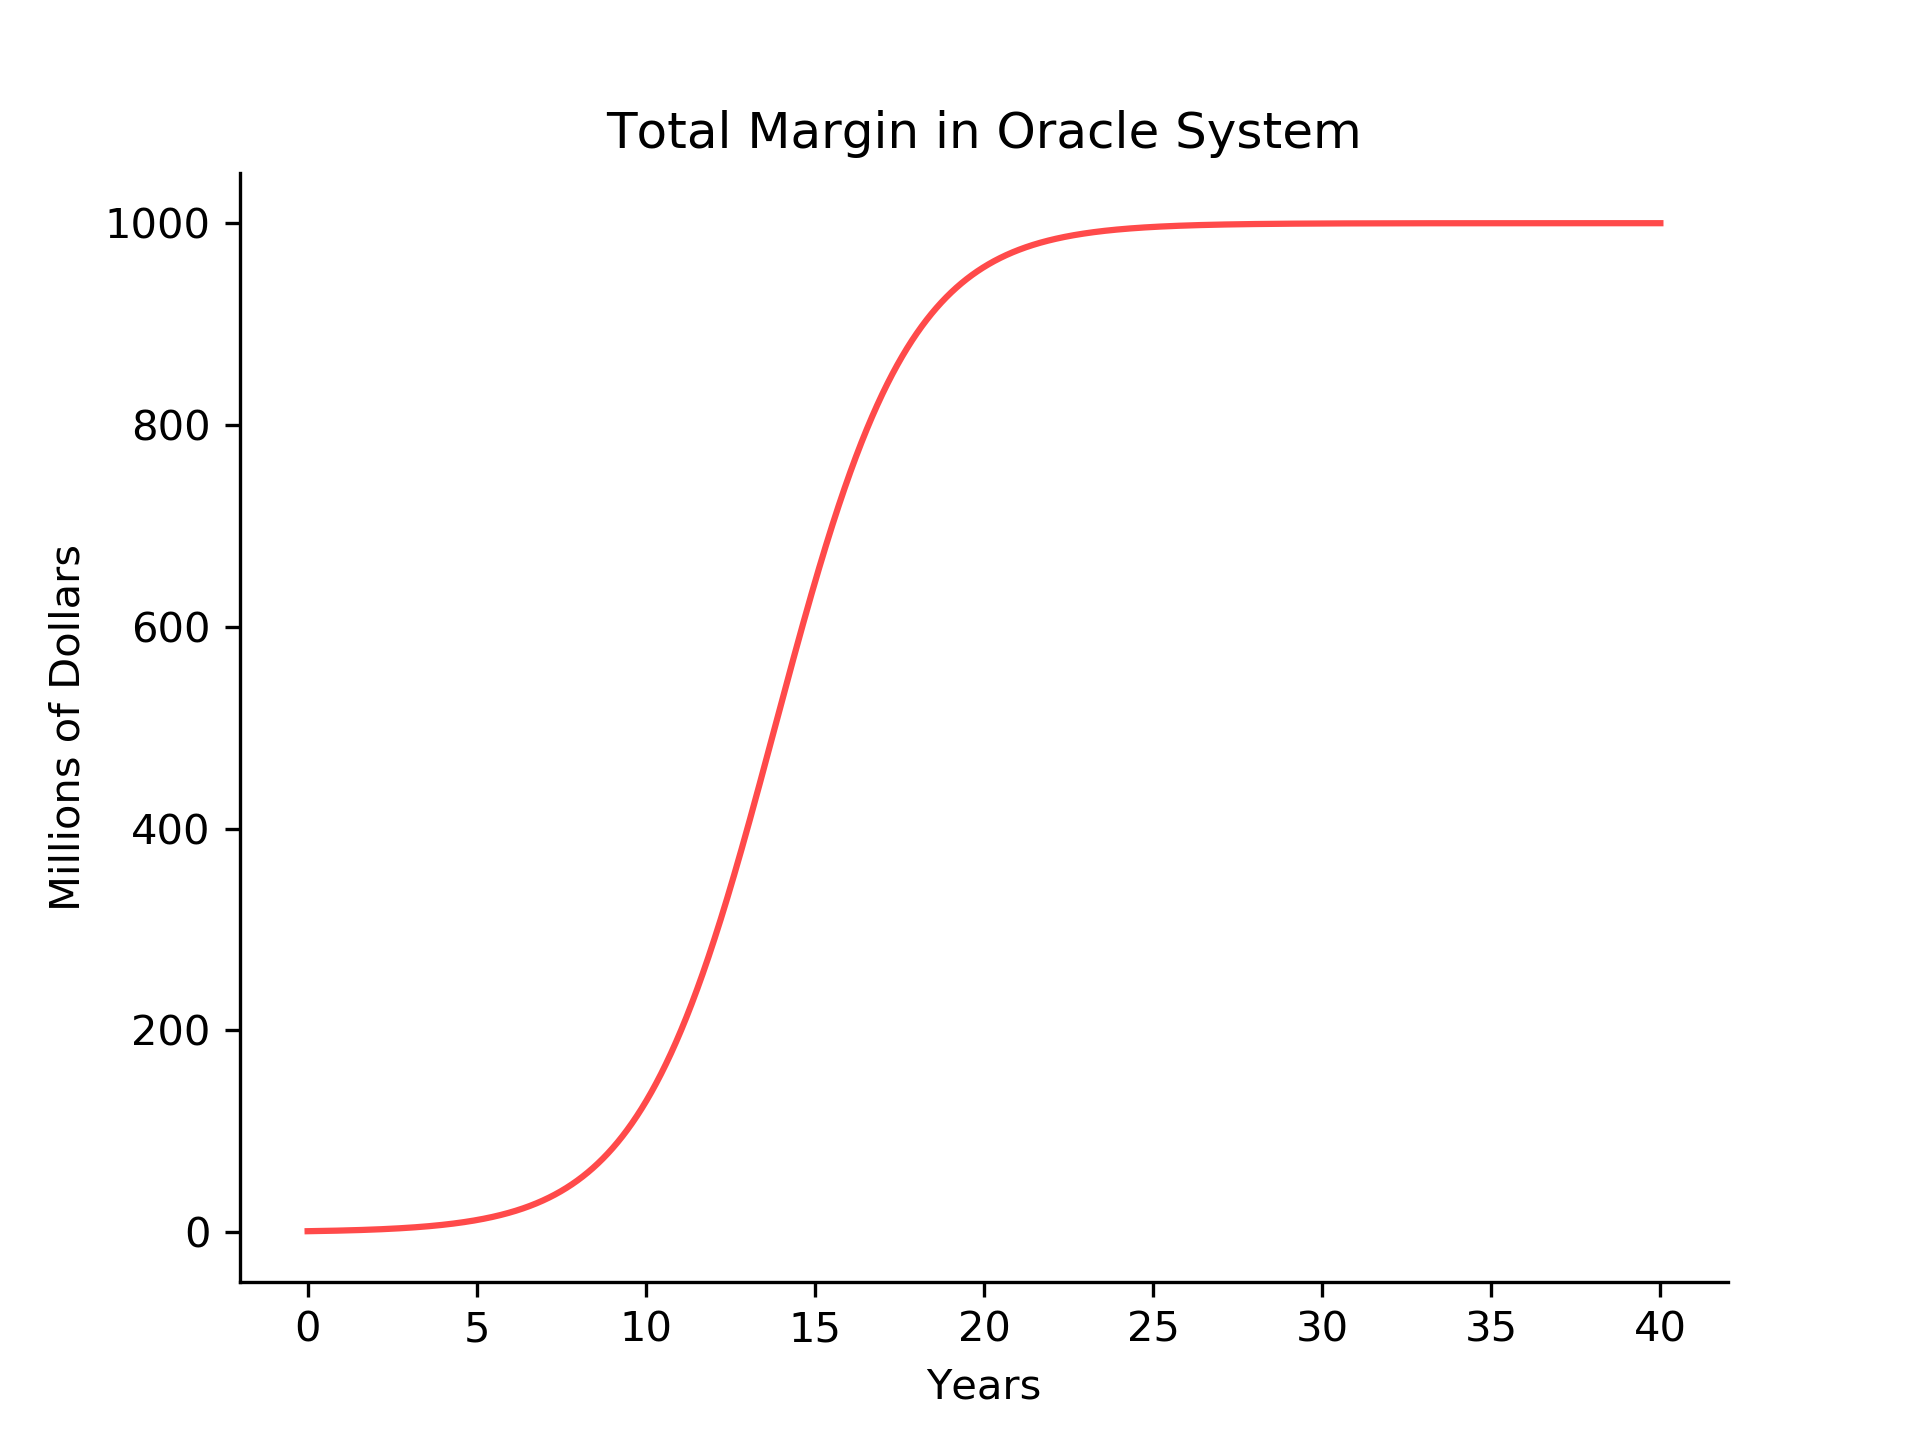
\includegraphics{./TaxationPlanImages/MarginGrowth.png}}
    \label{fig:dg_margin_growth}
  \end{figure}
\end{center}


We assume that we'd like to charge the minimum amount of taxes while maintaining the system's
incorruptibility. This produces the following program:

\begin{align*}
  \min_{T_t} \; &E \left[ \sum_{t=0} \left(\frac{1}{1 + r} \right)^t T_t \right] \\
  &\text{subject to} \\
  PfC_t &\leq \frac{1}{2} P_t S_t = \frac{1}{2} E \left[ \sum_{s=0} \left(\frac{1}{1 + r}\right)^s  X_{t + s} \right] \\
  X_{t} &= T_t \\
  0 &\leq T_t \\
  T_t &\leq \bar{\tau} \bar{M} \\
  M_{t+1} &= M_{t} + g M_{t} \left(1 + \frac{M_t}{\bar{M}} \right)
\end{align*}

The way that we solve this is that we start at $s$ such that $M_s \approx \bar{M}$. At this point,
we have arrived in the steady state and the tax rate implemented will be $T_t = \bar{\tau} M_t$. We
can then step back by one period to $t = s - 1$ and compute what the required $X_t$ in that period
would be. We can proceed to step this back until we reach our initial condition of $M_0$ which
traces out a path of tax collections. This process generates a sequence of taxes that look like
Figure \ref{fig:dg_tax_growth}.

\begin{center}
  \begin{figure}[H]
    \scalebox{0.65}{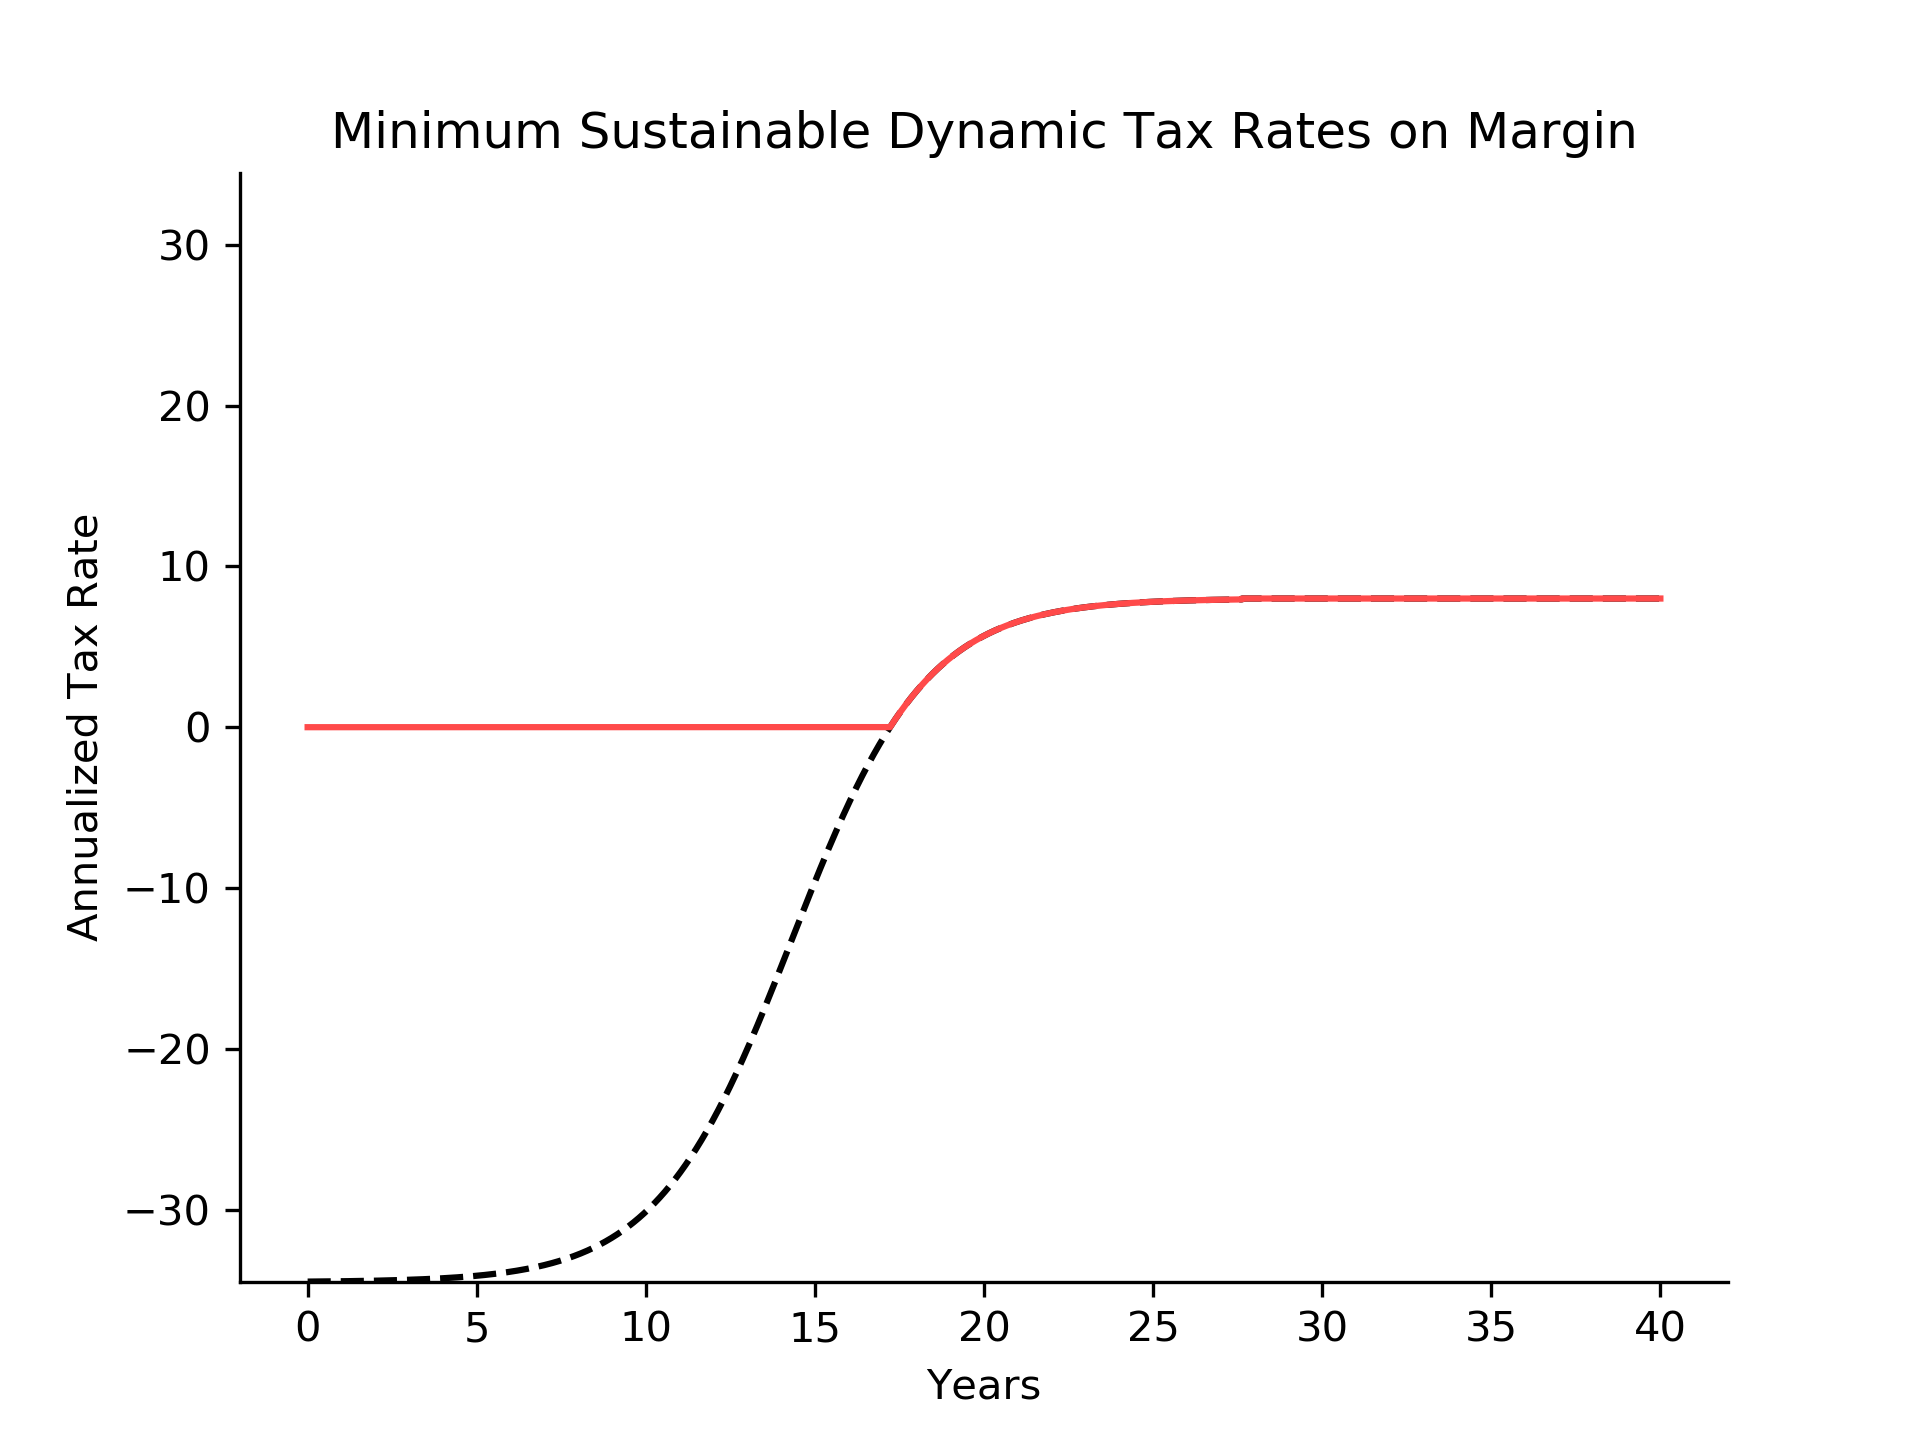
\includegraphics{./TaxationPlanImages/TaxRates.png}}
    \label{fig:dg_tax_growth}
  \end{figure}
\end{center}

The interesting observation that corresponds to this process is that the tax rates can start
relatively low and stay low for a prolonger period of time simply because people know that there
will be growth in the system --- This future promise of increased buybacks in the future is
enough to secure the system while it is small. However, this depends drastically on the fact that
margin grows deterministically and, in practice, the future growth may not be as certain as
predicted in this model (but we only need that the marginal token holder believes in the growth).
